\documentclass[a4paper,11pt]{scrartcl}

\usepackage[margin=1in]{geometry}
\usepackage[scaled]{helvet}
\usepackage[T1]{fontenc}
\usepackage[onehalfspacing]{setspace}
\usepackage[utf8]{inputenc}
\usepackage{amsmath}
\usepackage{mathptmx}
\usepackage{courier}
\usepackage{graphicx}
\usepackage{ulem}
\usepackage{bookmark}
\usepackage{paralist}
\usepackage{ngerman}
\usepackage{fancyhdr}
\usepackage{float}
\usepackage{array}
\usepackage{lipsum}


\graphicspath{ {../img/} }
\renewcommand\familydefault{\sfdefault}




\pagestyle{fancy}
\fancyhf{}
\renewcommand{\headrulewidth}{0pt}
\fancyfoot[C]{
\includegraphics[width=\textwidth]{Polygon_gruen}\\ \thepage}


\rhead{
\includegraphics[width=\textwidth]{LogoHeader}}
\setlength\headheight{30pt}
\setlength\footskip{15pt}

\begin{document}
\renewcommand*{\arraystretch}{1.2}
\pagenumbering{gobble}
\begin{titlepage}
    \begin{center}
        \vspace*{1cm}\Huge
        \textbf{Produktdokumentation}\par                
        \vspace{0.5cm}\LARGE        
        Software Engineering II\par           
        \vspace{2cm}
        
\includegraphics[width=0.5\textwidth]{OptimaLogo_long}\par   
        \vspace{1cm}
        \textbf{Projekttitel: BonoboBoard}\par        
        \vfill\Large   
        Jakob Hutschenreiter (1419081)\\Jiesen Wang (9839152)\\Nick Kramer (3122448)\\Patrick Küsters (9815596)\\Peter Moritz Hinkel (2783930)\par
        %\vspace{2cm}  
        %
\includegraphics[width=0.5\textwidth]{Bonobo_Logo}\par        
        \vspace{2cm}
        DHBW Mannheim\\
        \today     
    \end{center}
\end{titlepage}

\section*{Änderungshistorie}
\begin{table}[h]
	\begin{tabular}{@{} p{20mm} p{25mm} p{25mm} p{75mm}}
		\textbf{Revision} & \textbf{Datum} & \textbf{Autor(en)} & \textbf{Beschreibung}\\
		1.0 & 18.03.2022 & NK & A: 1, 2, 3\\
	\end{tabular}
\end{table}
\noindent
Abkürzungen: Hinzugefügt/Added (A), Änderung/Changed (C), Löschung/Deleted (D)
\vspace{2cm}
\tableofcontents
\newpage
\pagenumbering{arabic}

		%------------------------------------------------------------
		%-----  -----  ----- Begin actual content -----  -----  -----
		%------------------------------------------------------------
\section{Motivation und Grundlagen}\label{Grundlagen}
Dieses Dokument dient zur Beschreibung der Abläufe, die nötig sind, um das BonoboBoard lokal zu installieren und auszuführen. Auf den Aufbau des Software-Produkts wird hier nicht mehr eingegangen. Bitte ziehen Sie dafür die etwaigen anderen Dokumente heran.\\
Die nachfolgende Beschreibung wurde auf Basis folgender Abhängigkeiten erstellt:
\begin{table}[H]
\begin{tabular}{|p{5cm}|p{5cm}|}
\hline
\textbf{Software/Library} & \textbf{Version} \\ \hline
	Docker & 20.10.12, Build e91ed57 \\ \hline
	Docker Compose & 2.2.3\\ \hline
	Docker Desktop & 4.5.1 (74721)\\ \hline
%	PyCharm & 2021.3.2 \\ \hline
%	VisualStudio Code & 1.64.2 \\ \hline
%	Python & 3.9 \\ \hline	
%	Django &  4.0.2\\ \hline
%	Django Tables & 2.4.1 \\ \hline
%	dj-database-url & 0.5.0 \\ \hline
%	Gunicorn & 20.1.0 \\ \hline
%	Beautiful Soup & 4.8.2 \\ \hline
%	Requests & 2.27.1 \\ \hline
%	iCalendar & 4.0.9 \\ \hline
%	Pandas & 1.4.0 \\ \hline
%	lxml & 4.5.0 \\ \hline
%	SQLAlchemy & 1.4.31 \\ \hline
%	asgiref & 3.4.1 \\ \hline
%	autopep8 & 1.6.0 \\ \hline
%	pycodestyle & 2.8.0 \\ \hline
%	python-decouple & 3.5 \\ \hline
%	pytz & 2021.3 \\ \hline
%	sqlparse & 0.4.2 \\ \hline
%	toml & 0.10.2 \\ \hline
%	Unipath & 1.1 \\ \hline
%	whitenoise & 5.3.0 \\ \hline
\end{tabular}
\end{table}
\noindent
Bitte stellen Sie sicher, dass Sie die genannten Voraussetzungen erfüllen, anderweitig kann nicht sichergestellt werden, dass die Installation auf Ihrem System ordnungsgemäß funktioniert.\\

\noindent Wenn Sie das Produkt lediglich nutzen möchten, können Sie die Installationsdokumentation überspringen und direkt zu Abschnitt \ref{Kurzanleitung} wechseln. Kein Nutzer muss das BonoboBoard lokal installieren, die aktuelle Version kann immer unter \url{https://bonoboboard.de/} gefunden und genutzt werden. Falls Sie das Produkt weiterentwickeln möchten oder eine lokale Installation anstreben, ist mit Abschnitt \ref{Installationsdokumentation} fortzufahren. 

\section{Installationsdokumentation}\label{Installationsdokumentation}
Durch die Nutzung von Containern unter Docker lässt sich die Installation in einigen wenigen Schritten behandeln.
\subsection{Beziehen des Source-Code}
Der Source-Code wird auf GitHub gepflegt\footnote{https://github.com/Software-Engineering-DHBW/BonoboBoard}. Da es sich um ein öffentliches Repository handelt, kann der Code ohne weitere Authentifizierung lokal geklont werden. Für eine detaillierte Anleitung des Klon-Prozesses wird auf die offizielle Dokumentation von GitHub verwiesen\footnote{https://docs.github.com/en/repositories/creating-and-managing-repositories/cloning-a-repository}.\\
Ist das Klonen abgeschlossen, sollte folgende Struktur auf der ersten Ebene des Projekts zu finden sein:
\begin{figure}[H]
\begin{center}
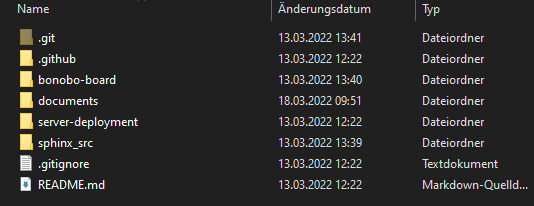
\includegraphics[width=0.8\textwidth]{folder_repo_1}
\caption{Ordnerstruktur des heruntergeladenen Projekts}
\label{img:folder_1}
\end{center}
\end{figure}

\subsection{Installation und Start der Docker Container}
%TODO maybe Änderung des Ports falls 80 belegt?
Dieser Abschnitt beschreibt den Ablauf, wie die Docker-Umgebung aufgebaut und gestartet wird. Dazu muss in den Ordner \textit{bonobo-board} (siehe dritter Ordner von oben in Abbildung \ref{img:folder_1}) gewechselt werden. Darin befindet sich eine Datei mit dem Namen \textit{docker-compose.yaml} und ein Dockerfile. Sollten diese nicht vorhanden sein, ist entweder nicht der richtige Ordner ausgewählt oder beim Herunterladen der Dateien sind Fehler aufgetreten. Hier eine Abbildung des Verzeichnisses zum Vergleich:
\begin{figure}[H]
\begin{center}
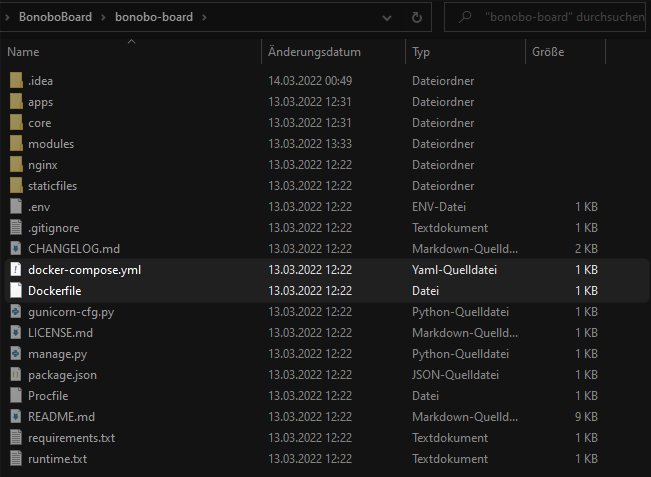
\includegraphics[width=0.8\textwidth]{folder_repo_2}
\caption{Struktur in \textit{bonobo-board}}
\label{img:folder_1}
\end{center}
\end{figure}

\noindent Nun muss ein Terminal in diesem Ordner gestartet werden.\\
Im Terminal ist der Befehl \texttt{docker-compose up} auszuführen. Alternativ kann der Befehl \\\texttt{docker-compose up -d} ausgeführt werden, wenn die Kommandozeile nach dem ausführen des Befehls nicht blockiert sein soll. In diesem Fall laufen die gestarteten Container im Hintergrund weiter. Abbildung \ref{img:docker-compose} zeigt beispielhaft die Ausgabe der Befehle in der Kommandozeile.\\ 
Bei Fehlermeldungen ist sicherzustellen, dass der docker-deamon läuft (Windows: läuft Docker-Desktop?) oder alle Voraussetzungen (siehe \ref{Grundlagen}) erfüllt sind.
\begin{figure}[H]
\begin{center}
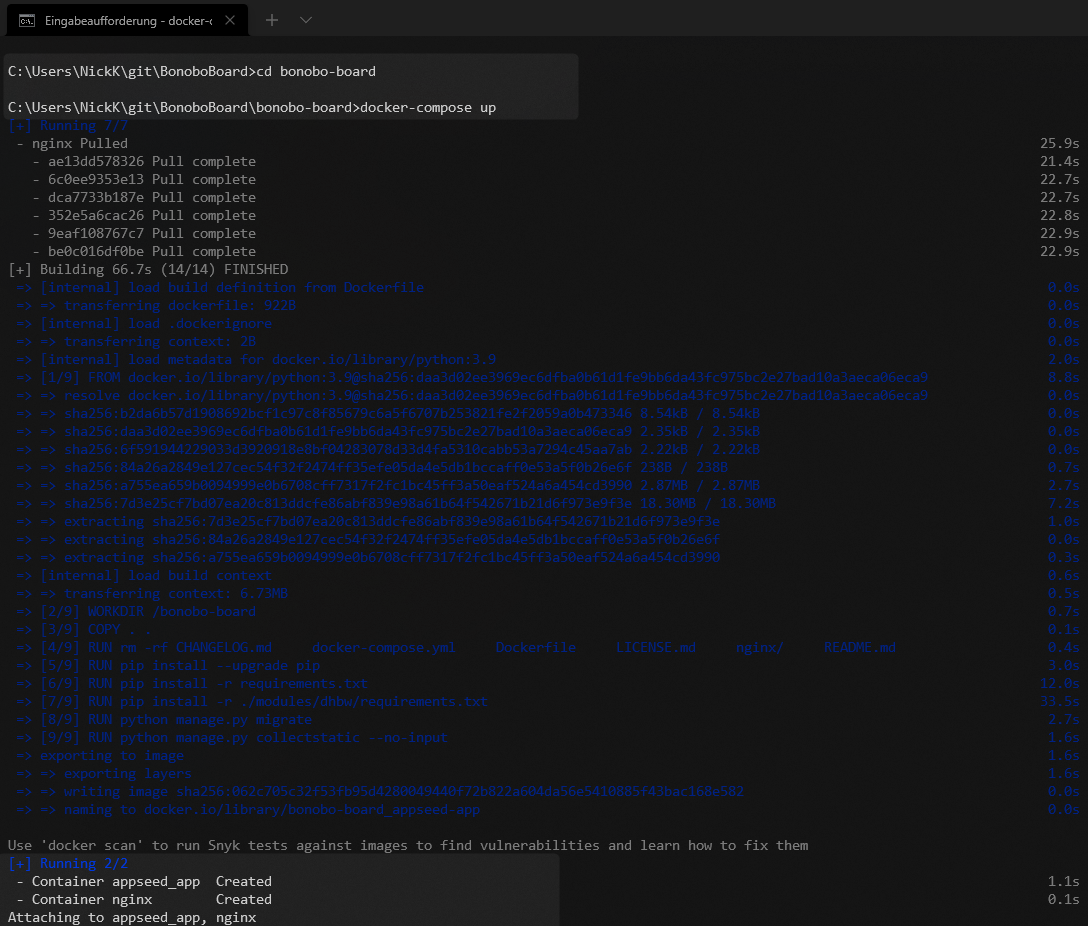
\includegraphics[width=\linewidth]{docker-compose}
\caption{docker-compose in der Kommandozeile}
\label{img:docker-compose}
\end{center}
\end{figure}

\subsection{Darstellung im Webbrowser}
Da die Container nun gestartet sind, ist zu prüfen ob alles funktioniert und die Website lokal erreichbar ist. Dafür ist ein Webbrowser nach Wahl zu öffnen und \url{http://localhost:80/} einzugeben. Es sollte sich die Website, wie in Abbildung \ref{img:darstellung} dargestellt, öffnen.
\begin{figure}[H]
\begin{center}
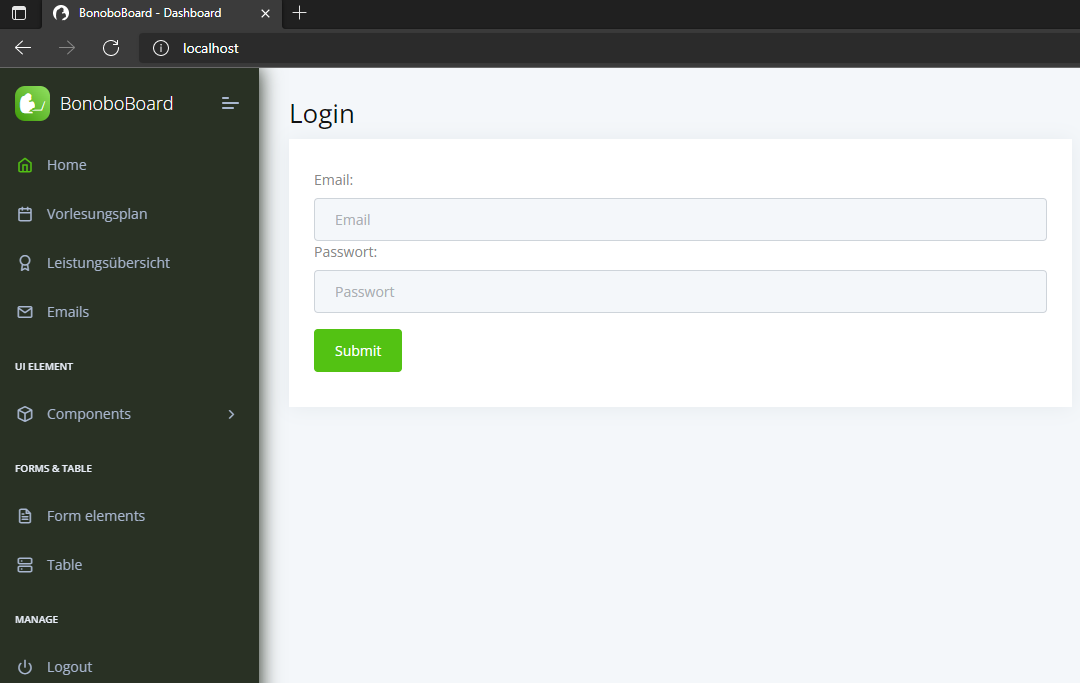
\includegraphics[width=0.8\textwidth]{webbrowser_localhost}
\caption{Darstellung im Browser}
\label{img:darstellung}
\end{center}
\end{figure}
\noindent
Damit ist die lokale Installation des BonoboBoard abgeschlossen.\\

\noindent
Haben alle Schritte vorab funktioniert und die Darstellung funktioniert trotzdem nicht, ist sicherzustellen, dass kein anderer Dienst Port 80 belegt. Unter Windows kann dies mit Hilfe der Kommandozeile und des Taskmanagers überprüft werden. Dazu ist der Befehl \texttt{netstat -ano -t tcp} auszuführen und die Zeile zu lokalisieren, in der die lokale Adresse 0.0.0.0:80 durch die remote Adresse 0.0.0.0:0 abgehört wird. Die PID am Ende dieser Zeile kann im Task-Manager auf eine Anwendung zurückgeführt werden. In Abbildung \ref{img:netstat} ist dies dargestellt. In diesem Fall wird die Website ordnungsgemäß dargestellt. Benutzt ein anderer Prozess (außer Docker-Desktop) diesen Port, ist dieser zu terminieren.
\begin{figure}[H]
\begin{center}
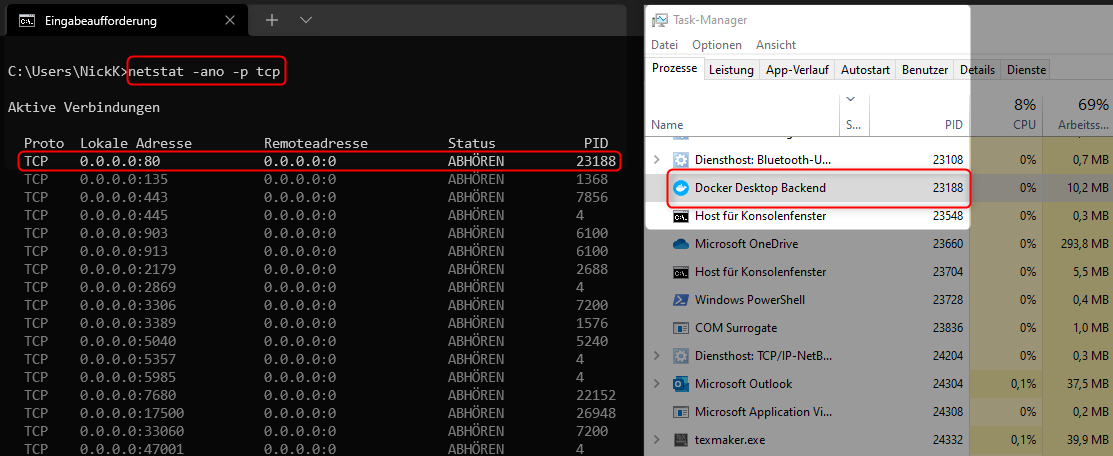
\includegraphics[width=\textwidth]{netstat_port80}
\caption{Überprüfung des lokalen Port 80}
\label{img:netstat}
\end{center}
\end{figure}
\section{Kurzanleitung}\label{Kurzanleitung}
Herzlich willkommen beim BonoboBoard! Danke, dass Sie sich für ein Produkt von Optima Connect entschieden haben. 

\bigskip
In dieser Kurzanleitung werden wir sie mit den grundlegenden Funktionen Ihres persönlichen DHBW-Dashboards vertraut machen, sodass Sie bereits in Kürze Ihren Workflow mit BonoboBoard optimieren können.

\subsection{Anmeldung}
Um das BonobobBoard benutzen zu können, gehen sie im Webbrowser Ihrer Wahl auf \url{https://bonoboboard.de} oder - falls Sie eine lokale Installation verwenden - auf \url{http://localhost:80/}. Von dort aus gelangen Sie zum Login (siehe Abb. \ref{img:login}).

\begin{figure}[H]
	\begin{center}
		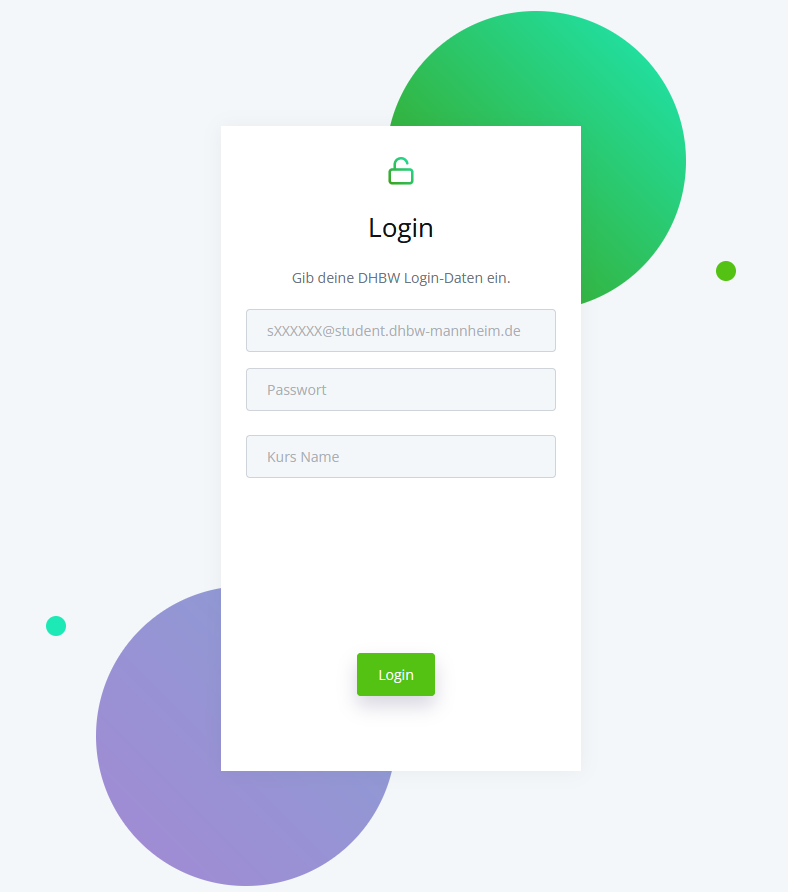
\includegraphics[width=0.8\textwidth]{login}
		\caption{BonoboBoard - Login}
		\label{img:login}
	\end{center}
\end{figure}
\noindent

Geben Sie nun dort Ihre DHBW-Mailadresse (s-Adresse) und Ihr Passwort, dass sie für Ihren DHBW-Account verwenden, ein. Keine Sorge - Ihr Passwort wird weder lokal noch auf unserem Server gespeichert. Auch nicht als Hash. Wir verwenden es lediglich, um eine Verbindung, mit den DHBW-Services aufzubauen. Wird diese Verbindung geschlossen, müssen sie sich allerdings neu anmelden.

\bigskip
Anschließend geben Sie noch Ihre Kursbezeichnung an. Beispielweise \frqq{}TINF19 IT2\flqq{}. Achten Sie bitte auf das Leerzeichen zwischen Semester- und Kursbezeichnung. Oder verwenden sie die Autovervollständigung (siehe Abb. \ref{img:autocomplete}).
\begin{figure}[H]
	\begin{center}
		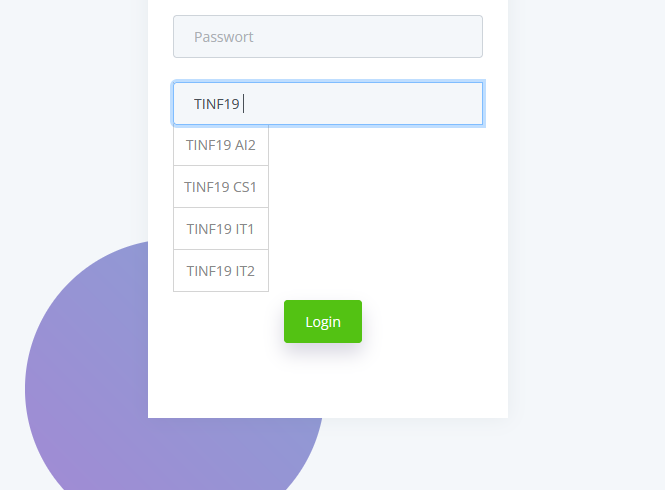
\includegraphics[width=0.8\textwidth]{autocomplete}
		\caption{BonoboBoard - Kusrauswahl}
		\label{img:autocomplete}
	\end{center}
\end{figure}
\noindent


		%------------------------------------------------------------
		%-----  -----  ------ End actual content ------  -----  -----
		%------------------------------------------------------------
\end{document}